
This section explains a general dataflow and the necessary steps to get data from an external source into a vectorized form. It will be held short giving intuition about a general setup, necessary preprocessing steps and the various problems that arise.

\section{Pipeline}
  A data pipeline for text data has various modules of interest. Where do we get the textutal content from? How is it stored? How is it preprocessed? What intermediate representations are useful? How do we handle the ongoing stream of input? The system that was developed for this thesis which is an early version is currently called ``News-Clusty''. Scraping, preprocessing and clustering are in place. There is a command line interface to interact with scraping and preprocessing. Currently it is an open question how to incorporate clustering schemes by a command line. The summarization and output generation is yet an open topic.

  \begin{figure}[h!]
    \centering
      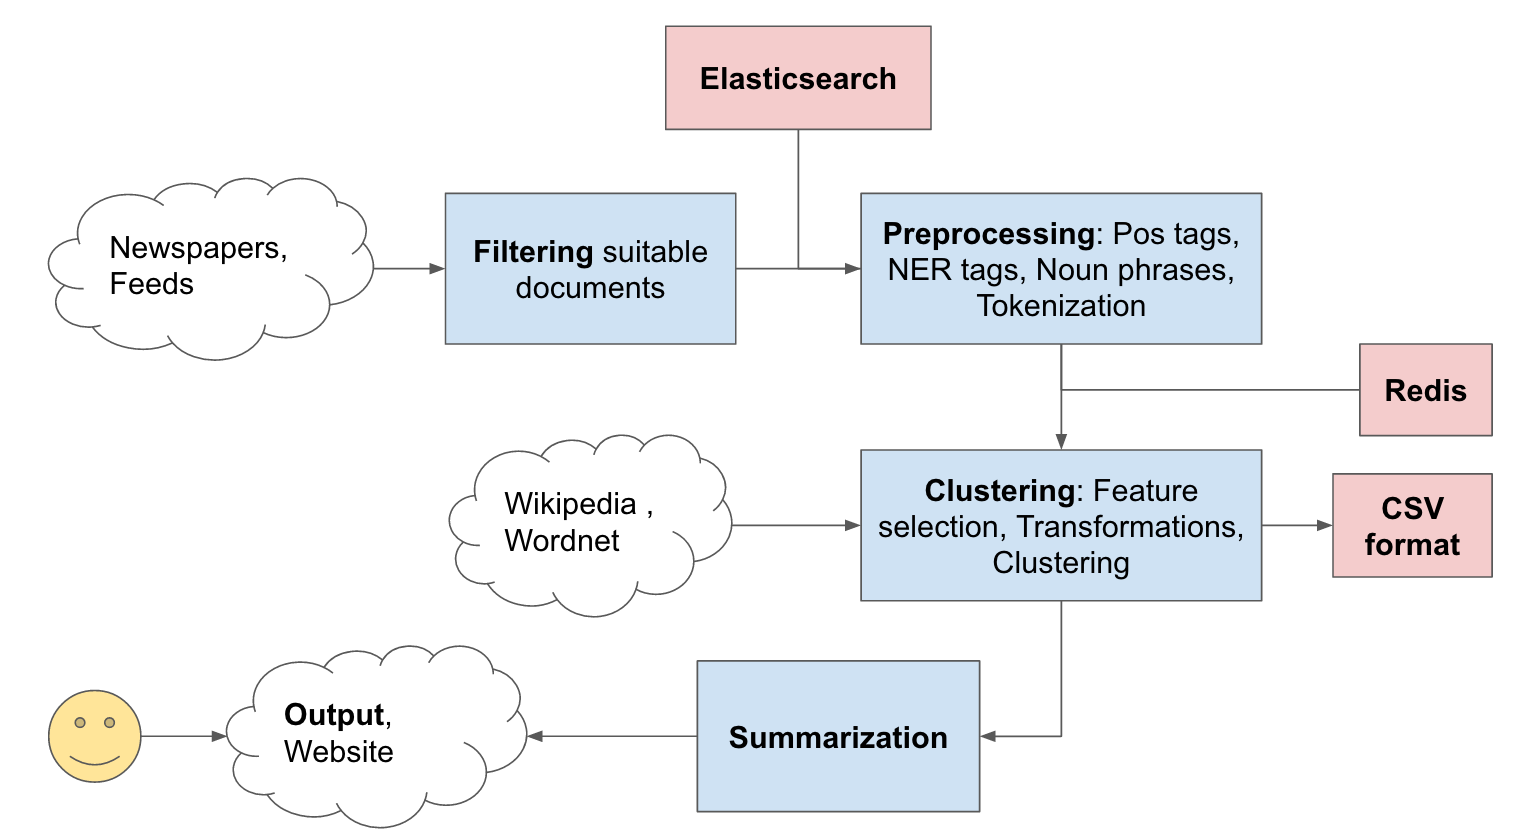
\includegraphics[width=0.7\textwidth]{news_clusty.png}
      \caption{"News-Clusty pipeline"}
      \label{news_clusty}
  \end{figure}

  The Columbia Newsblaster System by \cite{ColumbiaMultiDoc2001} is a very good point of reference. The core components of this system are:

  \begin{enumerate}
    \item \emph{Scraping} - get articles from the internet or predefined news sites and persist the raw content of a site. Here it is crucial to identify if a page is actually an article and if the desired content is correctly encoded, contains the correct language (if not multilingual), has a certain length, is not an advertisement. It is also possible to extract as much meta information as possible, like authors, meta keywords, keywords, categories, publishing dates, tags and links.

    \item \emph{Preprocessing} - extracting the raw content from html, xml or any kind of source that is found is a major part of preprocessing articles. Certain preconditions hold before preprocessing but might not be afterwards. If the html is stripped, is the text still long enough? A document in it's raw form can then be processed by stripping stop words, spell correcting the words and tokenize the content. Tokenization can either be by paragraph, sentence or word. If neeeded it is also recommended to store syntactical constructs like named entities, noun phrases and pos tags. Often when dealing with a lot of data it is no option to use these when doing actual cluster analysis as each of those often require several seconds per article to finish.

    \item \emph{Routing} - the router is an engine that detects if the input is a single event, a multi-event, person centered or something entirely different ``other''. A single event is about the same topic like the earthquake in Nepal. A multi-event are events at differentt times, palces and humans but with the same content. A person-centered view is often a biography for instance when the U.S. elections take place lots of candidates are interviewed about their opinions. This view makes it possible to make different assumptions about how articles should be summarized in case of single events or person centered events.

    \item \emph{Clustering} - The clustering primarily has several transformations to do. First  feature selection, by picking features that are of most interest in any kind of clustering scheme. Then if desired enhancing the features by definitions of Wikipedia or by projecting words of a document into corresponding hypernyms or hyponyms via Wordnet ontologies. The last step could be to stem or lemmatize the features. After this documents need to be lifted into vector space, topic models can be extracted, distances between documents calculated,dimensionalities reduced, normalization or scaling applied and the results clustered by different algorithms. The output is fed into a summarization engine.

    \item \emph{Summarization} - In summarization preclustered documents of interest, possibly with a lot of meta information can be summarized. Either by single document or by multiple documents that where in the same cluster. If assignments are soft, possible cluster overlaps can take place too. 

    \item \emph{Output generation} - Here it is only a matter of visualizing the results of a summarization engine. For instance a website with rendered html.
  \end{enumerate}

  The routing is something that could really boost performance. By identifying which documents are part of different summarization schemes it is much easier to incorporate language specific strategies. Due to time constraints this is an open question and should be investigated further.

\section{Python and Libraries}
  News-Clusty is entirely written in the programming language Python and a well versed collection of libraries. Persistence is in Elasticsearch, Redis and simple compressed files on a filesystem. The Named Entity Tagger by Stanford is involved as well and the Conll Noun phrase extractor. 

  \paragraph{Python} is a dynamic, object oriented higher level programming language with a rich environment for scientific computing. Python incoporates many different styles and assumptions, thusly leading to a variety of programming paradigms between object oriented and functional programming. From the Zen of Python: ``Beautiful is better than ugly. Explicit is better than implicit. Simple is better than complex.''. For a proper introduction to Python see \cite{NltkPython}.

  \paragraph{Persistence} - Long standing persistence of articles are held in Elasticsearch. Redis is used as a cache for different feature selection strategies. Several runs with the same feature selection strategy but different clustering algorithm settings will get the documents from Elasticsearch at first and successively from Redis. While databases have huge advantages if you would like to get certain types of document by search criterias, they are a overhead when accessing all files at once. If for a particular reason a whole dataset must be used it is advised to use some of the pickeling tools that will compress data into large files. Input and output on filesystems is much faster if you do not need to query the data. This holds true as long as a single node filesystem is involved. Elasticsearch for instance has its powers by leveraging clusters of servers (nodes) and is at its core meant to be a distributed system. The indices for Elasticsearch are build up as dates:

    \begin{equation}
      20150701/article/title_id = document
    \end{equation}

  for Redis respectively:

    \begin{equation}
      20150701-title_id = feature vector
    \end{equation}

  \paragraph{Libraries} - A general word on libraries. Throughout this thesis most of the components were build on abstractions provided by libraries that were not in any part, build by the system designers. That means the system leverages linear algebra, feature selection strategies and clustering algorithms from scipy (especially numpy and sklearn) see \cite{ScikitLearn}. It uses natural language analysis tools from the nltk by \cite{NltkPython}. Moreover named entitiy recognition by the StanfordNLP group, noun phrase extraction by Conll, word ontologies by Wordnet, Knowledge and dictionaries by Wikipedia.



